\documentclass[tikz,border=2pt]{standalone}
\usepackage{amsmath,amssymb}
\usepackage{tikz}
\usetikzlibrary{positioning, arrows.meta}

\begin{document}
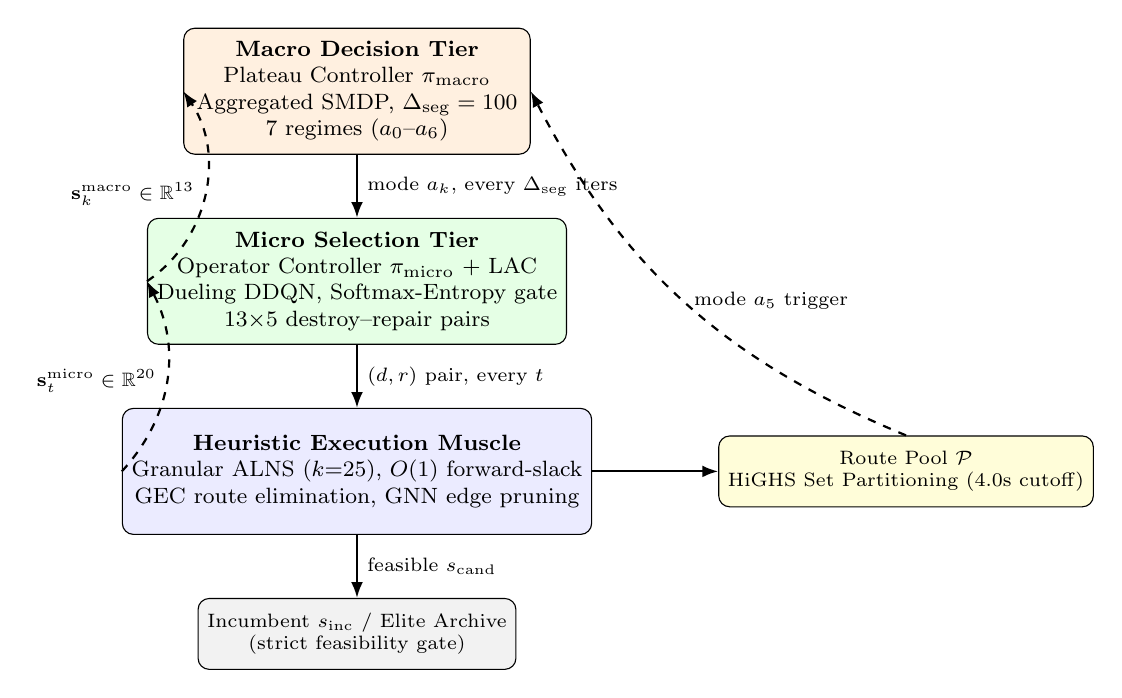
\begin{tikzpicture}[
  node distance=8mm and 16mm,
  tier/.style={draw, rounded corners, minimum width=4.4cm, minimum height=1.6cm, align=center, font=\footnotesize},
  comp/.style={draw, rounded corners, minimum width=3.6cm, minimum height=0.9cm, align=center, font=\scriptsize, fill=white},
  arr/.style={-{Latex[length=2mm]}, thick},
  fbarr/.style={-{Latex[length=2mm]}, thick, dashed}
]
  \node[tier, fill=orange!12] (macro) {\textbf{Macro Decision Tier}\\Plateau Controller $\pi_{\text{macro}}$\\Aggregated SMDP, $\Delta_{\text{seg}}=100$\\7 regimes ($a_0$--$a_6$)};
  \node[tier, fill=green!10, below=of macro] (micro) {\textbf{Micro Selection Tier}\\Operator Controller $\pi_{\text{micro}}$ + LAC\\Dueling DDQN, Softmax-Entropy gate\\13$\times$5 destroy--repair pairs};
  \node[tier, fill=blue!8, below=of micro] (heur) {\textbf{Heuristic Execution Muscle}\\Granular ALNS ($k$=25), $O(1)$ forward-slack\\GEC route elimination, GNN edge pruning};
  \node[comp, right=of heur, fill=yellow!15] (pool) {Route Pool $\mathcal{P}$\\HiGHS Set Partitioning (4.0s cutoff)};
  \node[comp, below=of heur, fill=gray!10] (inc) {Incumbent $s_{\text{inc}}$ / Elite Archive\\(strict feasibility gate)};

  \draw[arr] (macro) -- node[right, font=\scriptsize]{mode $a_k$, every $\Delta_{\text{seg}}$ iters} (micro);
  \draw[arr] (micro) -- node[right, font=\scriptsize]{$(d,r)$ pair, every $t$} (heur);
  \draw[arr] (heur) -- node[right, font=\scriptsize]{feasible $s_{\text{cand}}$} (inc);
  \draw[arr] (heur) -- (pool);
  \draw[fbarr] (heur.west) to[bend right=35] node[left, font=\scriptsize]{$\mathbf{s}_t^{\text{micro}}\in\mathbb{R}^{20}$} (micro.west);
  \draw[fbarr] (micro.west) to[bend right=45] node[left, font=\scriptsize]{$\mathbf{s}_k^{\text{macro}}\in\mathbb{R}^{13}$} (macro.west);
  \draw[fbarr] (pool.north) to[bend left=20] node[right, font=\scriptsize]{mode $a_5$ trigger} (macro.east);
\end{tikzpicture}
\end{document}
